% Created by tikzDevice version 0.12 on 2019-03-12 12:51:38
% !TEX encoding = UTF-8 Unicode
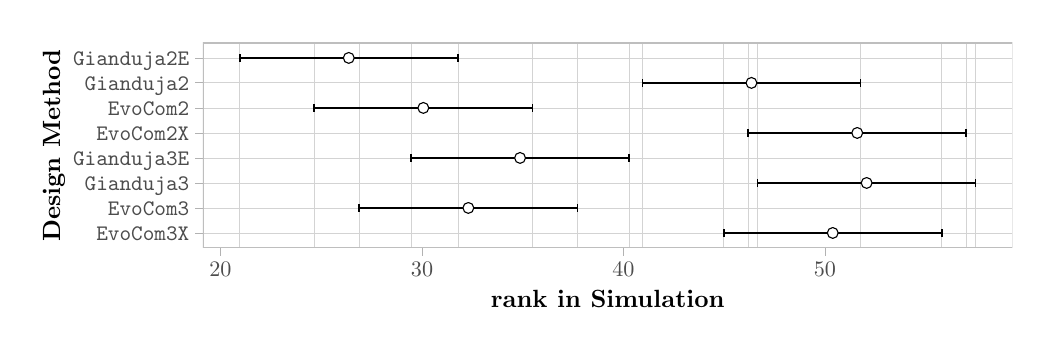
\begin{tikzpicture}[x=1pt,y=1pt]
\definecolor{fillColor}{RGB}{255,255,255}
\path[use as bounding box,fill=fillColor,fill opacity=0.00] (0,0) rectangle (361.35,108.41);
\begin{scope}
\path[clip] (  0.00,  0.00) rectangle (361.35,108.40);
\definecolor{drawColor}{RGB}{255,255,255}
\definecolor{fillColor}{RGB}{255,255,255}

\path[draw=drawColor,line width= 0.6pt,line join=round,line cap=round,fill=fillColor] (  0.00,  0.00) rectangle (361.35,108.40);
\end{scope}
\begin{scope}
\path[clip] ( 63.34, 28.81) rectangle (355.85,102.90);
\definecolor{fillColor}{RGB}{255,255,255}

\path[fill=fillColor] ( 63.34, 28.81) rectangle (355.85,102.90);
\definecolor{drawColor}{RGB}{211,211,211}

\path[draw=drawColor,line width= 0.3pt,line join=round] ( 63.34, 79.41) --
	(355.85, 79.41);

\path[draw=drawColor,line width= 0.3pt,line join=round] ( 63.34, 43.27) --
	(355.85, 43.27);

\path[draw=drawColor,line width= 0.3pt,line join=round] ( 63.34, 88.45) --
	(355.85, 88.45);

\path[draw=drawColor,line width= 0.3pt,line join=round] ( 63.34, 97.48) --
	(355.85, 97.48);

\path[draw=drawColor,line width= 0.3pt,line join=round] ( 63.34, 52.30) --
	(355.85, 52.30);

\path[draw=drawColor,line width= 0.3pt,line join=round] ( 63.34, 61.34) --
	(355.85, 61.34);

\path[draw=drawColor,line width= 0.3pt,line join=round] ( 63.34, 34.23) --
	(355.85, 34.23);

\path[draw=drawColor,line width= 0.3pt,line join=round] ( 63.34, 70.37) --
	(355.85, 70.37);

\path[draw=drawColor,line width= 0.2pt,line join=round] (182.37, 28.81) -- (182.37,102.90);

\path[draw=drawColor,line width= 0.2pt,line join=round] (339.16, 28.81) -- (339.16,102.90);

\path[draw=drawColor,line width= 0.2pt,line join=round] (300.93, 28.81) -- (300.93,102.90);

\path[draw=drawColor,line width= 0.2pt,line join=round] (155.42, 28.81) -- (155.42,102.90);

\path[draw=drawColor,line width= 0.2pt,line join=round] (198.63, 28.81) -- (198.63,102.90);

\path[draw=drawColor,line width= 0.2pt,line join=round] (330.30, 28.81) -- (330.30,102.90);

\path[draw=drawColor,line width= 0.2pt,line join=round] (342.55, 28.81) -- (342.55,102.90);

\path[draw=drawColor,line width= 0.2pt,line join=round] (217.32, 28.81) -- (217.32,102.90);

\path[draw=drawColor,line width= 0.2pt,line join=round] (103.58, 28.81) -- (103.58,102.90);

\path[draw=drawColor,line width= 0.2pt,line join=round] (260.37, 28.81) -- (260.37,102.90);

\path[draw=drawColor,line width= 0.2pt,line join=round] (222.15, 28.81) -- (222.15,102.90);

\path[draw=drawColor,line width= 0.2pt,line join=round] ( 76.64, 28.81) -- ( 76.64,102.90);

\path[draw=drawColor,line width= 0.2pt,line join=round] (119.84, 28.81) -- (119.84,102.90);

\path[draw=drawColor,line width= 0.2pt,line join=round] (251.51, 28.81) -- (251.51,102.90);

\path[draw=drawColor,line width= 0.2pt,line join=round] (263.77, 28.81) -- (263.77,102.90);

\path[draw=drawColor,line width= 0.2pt,line join=round] (138.53, 28.81) -- (138.53,102.90);
\definecolor{drawColor}{RGB}{0,0,0}

\path[draw=drawColor,line width= 0.6pt,line join=round] (182.37, 78.06) --
	(182.37, 80.77);

\path[draw=drawColor,line width= 0.6pt,line join=round] (182.37, 79.41) --
	(103.58, 79.41);

\path[draw=drawColor,line width= 0.6pt,line join=round] (103.58, 78.06) --
	(103.58, 80.77);

\path[draw=drawColor,line width= 0.6pt,line join=round] (339.16, 69.02) --
	(339.16, 71.73);

\path[draw=drawColor,line width= 0.6pt,line join=round] (339.16, 70.37) --
	(260.37, 70.37);

\path[draw=drawColor,line width= 0.6pt,line join=round] (260.37, 69.02) --
	(260.37, 71.73);

\path[draw=drawColor,line width= 0.6pt,line join=round] (300.93, 87.09) --
	(300.93, 89.80);

\path[draw=drawColor,line width= 0.6pt,line join=round] (300.93, 88.45) --
	(222.15, 88.45);

\path[draw=drawColor,line width= 0.6pt,line join=round] (222.15, 87.09) --
	(222.15, 89.80);

\path[draw=drawColor,line width= 0.6pt,line join=round] (155.42, 96.13) --
	(155.42, 98.84);

\path[draw=drawColor,line width= 0.6pt,line join=round] (155.42, 97.48) --
	( 76.64, 97.48);

\path[draw=drawColor,line width= 0.6pt,line join=round] ( 76.64, 96.13) --
	( 76.64, 98.84);

\path[draw=drawColor,line width= 0.6pt,line join=round] (198.63, 41.91) --
	(198.63, 44.62);

\path[draw=drawColor,line width= 0.6pt,line join=round] (198.63, 43.27) --
	(119.84, 43.27);

\path[draw=drawColor,line width= 0.6pt,line join=round] (119.84, 41.91) --
	(119.84, 44.62);

\path[draw=drawColor,line width= 0.6pt,line join=round] (330.30, 32.87) --
	(330.30, 35.59);

\path[draw=drawColor,line width= 0.6pt,line join=round] (330.30, 34.23) --
	(251.51, 34.23);

\path[draw=drawColor,line width= 0.6pt,line join=round] (251.51, 32.87) --
	(251.51, 35.59);

\path[draw=drawColor,line width= 0.6pt,line join=round] (342.55, 50.95) --
	(342.55, 53.66);

\path[draw=drawColor,line width= 0.6pt,line join=round] (342.55, 52.30) --
	(263.77, 52.30);

\path[draw=drawColor,line width= 0.6pt,line join=round] (263.77, 50.95) --
	(263.77, 53.66);

\path[draw=drawColor,line width= 0.6pt,line join=round] (217.32, 59.98) --
	(217.32, 62.69);

\path[draw=drawColor,line width= 0.6pt,line join=round] (217.32, 61.34) --
	(138.53, 61.34);

\path[draw=drawColor,line width= 0.6pt,line join=round] (138.53, 59.98) --
	(138.53, 62.69);

\path[draw=drawColor,line width= 0.4pt,line join=round,line cap=round,fill=fillColor] (142.97, 79.41) circle (  1.96);

\path[draw=drawColor,line width= 0.4pt,line join=round,line cap=round,fill=fillColor] (299.76, 70.37) circle (  1.96);

\path[draw=drawColor,line width= 0.4pt,line join=round,line cap=round,fill=fillColor] (261.54, 88.45) circle (  1.96);

\path[draw=drawColor,line width= 0.4pt,line join=round,line cap=round,fill=fillColor] (116.03, 97.48) circle (  1.96);

\path[draw=drawColor,line width= 0.4pt,line join=round,line cap=round,fill=fillColor] (159.24, 43.27) circle (  1.96);

\path[draw=drawColor,line width= 0.4pt,line join=round,line cap=round,fill=fillColor] (290.91, 34.23) circle (  1.96);

\path[draw=drawColor,line width= 0.4pt,line join=round,line cap=round,fill=fillColor] (303.16, 52.30) circle (  1.96);

\path[draw=drawColor,line width= 0.4pt,line join=round,line cap=round,fill=fillColor] (177.92, 61.34) circle (  1.96);
\definecolor{drawColor}{RGB}{190,190,190}

\path[draw=drawColor,line width= 0.6pt,line join=round,line cap=round] ( 63.34, 28.81) rectangle (355.85,102.90);
\end{scope}
\begin{scope}
\path[clip] (  0.00,  0.00) rectangle (361.35,108.41);
\definecolor{drawColor}{gray}{0.30}

\node[text=drawColor,anchor=base east,inner sep=0pt, outer sep=0pt, scale=  0.80] at ( 58.39, 76.66) {\texttt{EvoCom2}};

\node[text=drawColor,anchor=base east,inner sep=0pt, outer sep=0pt, scale=  0.80] at ( 58.39, 40.51) {\texttt{EvoCom3}};

\node[text=drawColor,anchor=base east,inner sep=0pt, outer sep=0pt, scale=  0.80] at ( 58.39, 85.69) {\texttt{Gianduja2}};

\node[text=drawColor,anchor=base east,inner sep=0pt, outer sep=0pt, scale=  0.80] at ( 58.39, 94.73) {\texttt{Gianduja2E}};

\node[text=drawColor,anchor=base east,inner sep=0pt, outer sep=0pt, scale=  0.80] at ( 58.39, 49.55) {\texttt{Gianduja3}};

\node[text=drawColor,anchor=base east,inner sep=0pt, outer sep=0pt, scale=  0.80] at ( 58.39, 58.58) {\texttt{Gianduja3E}};

\node[text=drawColor,anchor=base east,inner sep=0pt, outer sep=0pt, scale=  0.80] at ( 58.39, 31.48) {\texttt{EvoCom3X}};

\node[text=drawColor,anchor=base east,inner sep=0pt, outer sep=0pt, scale=  0.80] at ( 58.39, 67.62) {\texttt{EvoCom2X}};
\end{scope}
\begin{scope}
\path[clip] (  0.00,  0.00) rectangle (361.35,108.41);
\definecolor{drawColor}{gray}{0.70}

\path[draw=drawColor,line width= 0.3pt,line join=round] ( 60.59, 79.41) --
	( 63.34, 79.41);

\path[draw=drawColor,line width= 0.3pt,line join=round] ( 60.59, 43.27) --
	( 63.34, 43.27);

\path[draw=drawColor,line width= 0.3pt,line join=round] ( 60.59, 88.45) --
	( 63.34, 88.45);

\path[draw=drawColor,line width= 0.3pt,line join=round] ( 60.59, 97.48) --
	( 63.34, 97.48);

\path[draw=drawColor,line width= 0.3pt,line join=round] ( 60.59, 52.30) --
	( 63.34, 52.30);

\path[draw=drawColor,line width= 0.3pt,line join=round] ( 60.59, 61.34) --
	( 63.34, 61.34);

\path[draw=drawColor,line width= 0.3pt,line join=round] ( 60.59, 34.23) --
	( 63.34, 34.23);

\path[draw=drawColor,line width= 0.3pt,line join=round] ( 60.59, 70.37) --
	( 63.34, 70.37);
\end{scope}
\begin{scope}
\path[clip] (  0.00,  0.00) rectangle (361.35,108.41);
\definecolor{drawColor}{gray}{0.70}

\path[draw=drawColor,line width= 0.3pt,line join=round] ( 69.67, 26.06) --
	( 69.67, 28.81);

\path[draw=drawColor,line width= 0.3pt,line join=round] (142.49, 26.06) --
	(142.49, 28.81);

\path[draw=drawColor,line width= 0.3pt,line join=round] (215.30, 26.06) --
	(215.30, 28.81);

\path[draw=drawColor,line width= 0.3pt,line join=round] (288.11, 26.06) --
	(288.11, 28.81);
\end{scope}
\begin{scope}
\path[clip] (  0.00,  0.00) rectangle (361.35,108.41);
\definecolor{drawColor}{gray}{0.30}

\node[text=drawColor,anchor=base,inner sep=0pt, outer sep=0pt, scale=  0.80] at ( 69.67, 18.35) {20};

\node[text=drawColor,anchor=base,inner sep=0pt, outer sep=0pt, scale=  0.80] at (142.49, 18.35) {30};

\node[text=drawColor,anchor=base,inner sep=0pt, outer sep=0pt, scale=  0.80] at (215.30, 18.35) {40};

\node[text=drawColor,anchor=base,inner sep=0pt, outer sep=0pt, scale=  0.80] at (288.11, 18.35) {50};
\end{scope}
\begin{scope}
\path[clip] (  0.00,  0.00) rectangle (361.35,108.41);
\definecolor{drawColor}{RGB}{0,0,0}

\node[text=drawColor,anchor=base,inner sep=0pt, outer sep=0pt, scale=  0.90] at (209.60,  7.44) {\bfseries rank in Simulation};
\end{scope}
\begin{scope}
\path[clip] (  0.00,  0.00) rectangle (361.35,108.41);
\definecolor{drawColor}{RGB}{0,0,0}

\node[text=drawColor,rotate= 90.00,anchor=base,inner sep=0pt, outer sep=0pt, scale=  0.90] at ( 11.71, 65.86) {\bfseries Design Method};
\end{scope}
\end{tikzpicture}
